\documentclass[border=10pt]{standalone}

\usepackage{tikz}
\usepackage{tikzsymbols}
\usetikzlibrary{calc,patterns,shapes.geometric}

\def\centerarc[#1](#2)(#3:#4:#5){\draw[#1] ($(#2)+({#5*cos(#3)},{#5*sin(#3)})$) arc (#3:#4:#5);}

\begin{document}
	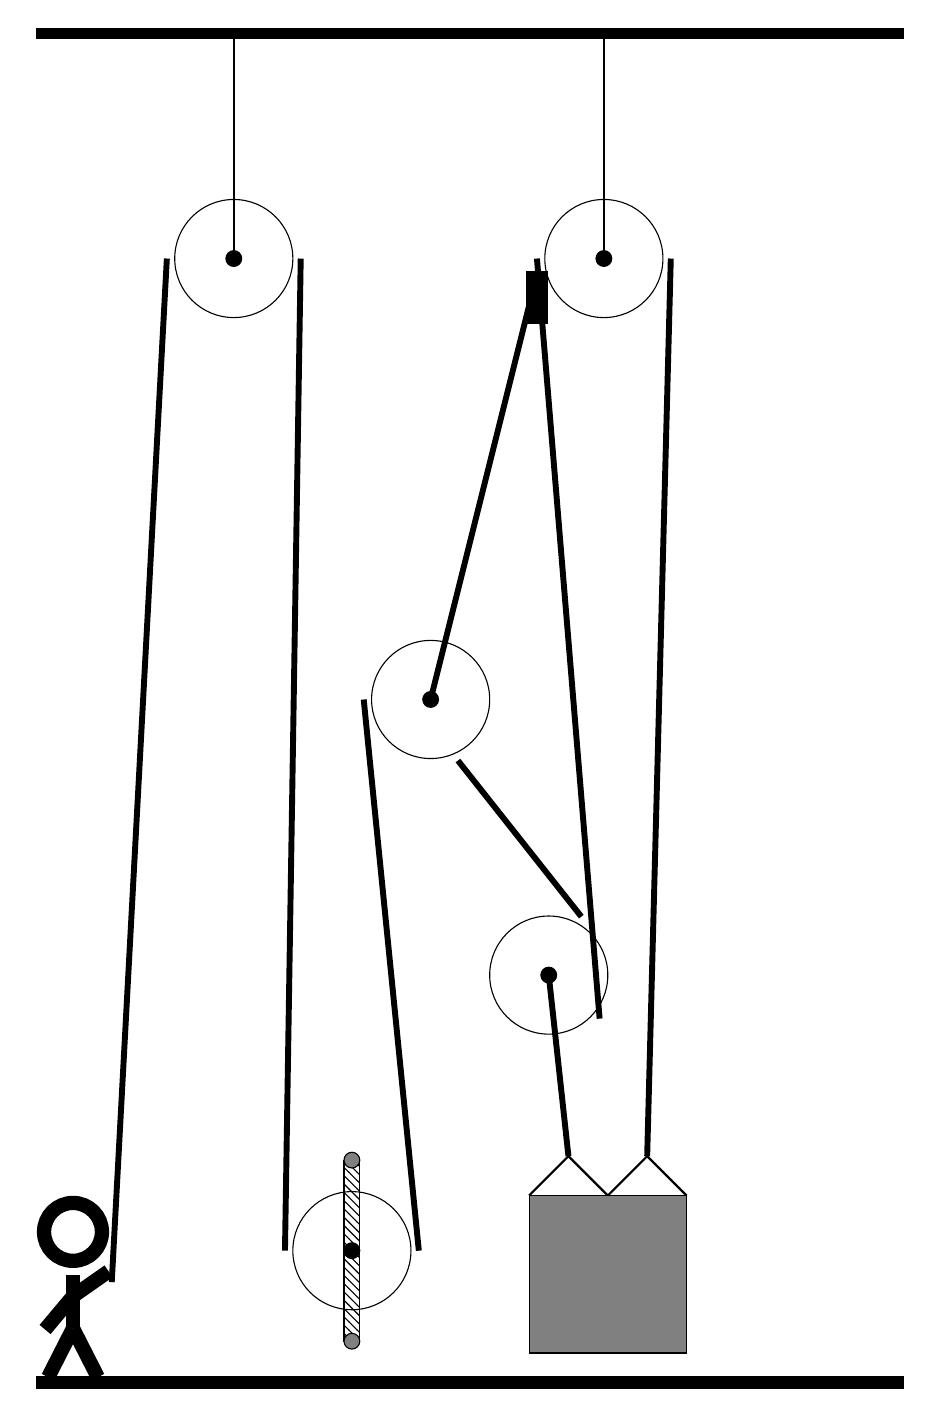
\begin{tikzpicture}
		%%%%% START %%%%%
		\draw[fill=black] (-6, 14) rectangle (5, 14.125);
		
		\draw (-1, 5.6) circle (0.75);
		\draw[fill=black] (-1, 5.6) circle (0.1);
		
		\draw (0.5, 2.1) circle (0.75);
		\draw[fill=black] (0.5, 2.1) circle (0.1);
		
		\draw (1.2, 11.2) circle (0.75);
		\draw[fill=black] (1.2, 11.2) circle (0.1);
		\draw[thick] (1.2, 11.2) -- (1.2, 14);
		
		\draw (-3.5, 11.2) circle (0.75);
		\draw[fill=black] (-3.5, 11.2) circle (0.1);
		\draw[thick] (-3.5, 11.2) -- (-3.5, 14);
		
		\draw (-2, -1.4) circle (0.75);
		\draw[fill=black] (-2, -1.4) circle (0.1);
		\draw[pattern=north west lines, pattern color=black] (-2.1, -0.25) rectangle (-1.9, -2.55);
		\draw[fill=black!50] (-2, -0.25) circle (0.1);
		\draw[fill=black!50] (-2, -2.55) circle (0.1);
		
		\draw[thick]  (0.25, -0.7) -- (0.75, -0.2) -- (1.25, -0.7) -- (1.75, -0.2) -- (2.25, -0.7);
		\draw[fill=black!50] (0.25, -0.7) rectangle (2.25, -2.7);
		\draw[line width=0.75mm] (-5.05, -1.8) -- (-4.35, 11.2);
		\centerarc[line width=0.75mm](-3.5, 11.2)(0:180:0.85);
		\draw[line width=0.75mm] (-2.65, 11.2) -- (-2.85, -1.4);
		\centerarc[line width=0.75mm](-2, -1.4)(180:360:0.85);
		\draw[line width=0.75mm] (-1.15, -1.4) -- (-1.85, 5.6);
		\draw[line width=0.75mm] (-1, 5.6) -- (0.35, 11.0);
		\draw[line width=0.75mm, fill=black](0.25, 10.4) rectangle (0.45, 11.0);
		\centerarc[line width=0.75mm](-1, 5.6)(-20:180:0.85);
		\draw[line width=0.75mm] (-0.653, 4.824) -- (0.914, 2.842);
		\centerarc[line width=0.75mm](0.5, 2.1)(160:380:0.85);
		\draw[line width=0.75mm] (1.146, 1.547) -- (0.35, 11.2);
		\draw[line width=0.75mm](0.5, 2.1) -- (0.75, -0.2);
		\centerarc[line width=0.75mm](1.2, 11.2)(0:180:0.85);
		\draw[line width=0.75mm] (2.05, 11.2) -- (1.75, -0.2);
		
		\node at (-5.5, -1.9) {\Strichmaxerl[10][50][35]};
		
		\draw[fill=black] (-6, -3) rectangle (5, -3.15);
		%%%%% END %%%%%
	\end{tikzpicture}
\end{document}